% ~~~~~~~~~~~~~~~~~~~~~~~~~~~~~~~~~~~~~~~~~~~~~~~~~~~~~~~~~~~~~~~~~~~~~~~~~~~~~
%                                 INTRODUCTION
% ~~~~~~~~~~~~~~~~~~~~~~~~~~~~~~~~~~~~~~~~~~~~~~~~~~~~~~~~~~~~~~~~~~~~~~~~~~~~~
\chapter{Introduction}\label{chap:1}
  \lhead{Chapter 1. \emph{Introduction}}
  In this chapter, there will be introduced existing approaches in solving
board games with agent based model, Quoridor game rules, chosen opponent model
to implement and Python programming langue.

\section{Agent based model}
Agent based model (ABM) is a paradigm in modeling systems comprised
of autonomous agents. Also, it is a class of computational models for
simulations of the actions and interactions between agents. Althought, there
are multiple definitions of what is considered agent [\cite{abm}], often, agent
is an identifiable component with reaction rules able to make independent
decisions (or behaviours) and sometimes with ability to learn and adapt to
the environment.

\section{Game theory}
TODO

\section{Markov decission process}
TODO

\section{A star}
TODO

\section{Alfa-beta pruning}
TODO

\section{Reinforcement Learning}
TODO

\section{Evolution methods and genetic algorithms}
TODO

\section{Q-Learning}
Q-Learning is reinforcement learning method. It learns an action-value
(q-value) function for any finite Markov decision process used to find
optimal policy for the agent. After it has learned the q-value function,
it can follow the optimal strategy by choosing best q-value. ?citation?
Algorithm is value iteration update for every observed state ?citation?:
\begin{equation}
Q_{t+1} \leftarrow Q_t(s_t, a_t) + \alpha \cdot (
    R_{t+1} + \gamma\cdot {\max_a}\,Q_t(s_{t+1}, a) - Q_t(s_t, a_t)
)
\end{equation}
where $Q_t(s_t, a_t)$ is old value, $\alpha$ is learning rate, $R_{t+1}$ is
reward after performing action $a_t$ in state $s_t$, $\gamma$ is discount
factor and $\underset{a}{\max}\,Q_t(s_{t+1}, a)$ is maximum optimal future
value.

\section{Perceptron}
\begin{wrapfigure}{l}{0.4\textwidth}
  \vspace*{-0.45cm}
  \centering
  \includegraphics[width=0.4\textwidth]{neural-net1.png}
  \vspace*{-1.45cm}
  \caption{ANN}
  \label{fig:network}
  \vspace*{-1.00cm}
\end{wrapfigure}

Artifitial neural network (ANN) is a family of models inspired by biological
neural networks used in computer science to approximate functions with
large number of inputs. Generally, artifitial neural network is presented
as a system of interconnected neurons exchanging messages between each
other. These connections have weights that can be adjusted based on
experience which makes the network capable of learning.

Perceptron is an algorithm for supervised learning of binary classifiers
where one neuron has multiple weighted inputs and single output. Single
perceptron can learn to decide between two linearly separable
classes. Multiple perceptrons in multiple layers (MLP) use arbitrary
activation function which makes it able to perform classification or
regression based on the activation function chosen.

\section{Perceptron estimating Q-learning}
\begin{wrapfigure}{r}{0.42\textwidth}
  \vspace*{-1.15cm}
  \begin{equation}
    \label{eqn:otheloqupdate}
    \hat{Q}^{new}\!\leftarrow\!r_t\!+\!{\gamma}{\max_a}\,\hat{Q}(s_{t+1},\!a)
    % \hat{Q}_t^{new}
    % \leftarrow r_t + {\gamma}{\max_a}\,\hat{Q}_{t+1}(s_{t+1}, a)
  \end{equation}
  \vspace*{-0.95cm}
\end{wrapfigure}

Main advantage of ANN is its ability to generalize. This is has been used
in game othello [\cite{othello}] with combining Q-learning so that network
has learned to estimate q-values for each state. Learning rate $\alpha$ has
not been directly used in iteration update (\ref{eqn:otheloqupdate}) since
ANN has also learning rate so it can be adjusted there.

\section{Quoridor Rules}
\begin{wrapfigure}{R}{0.4\textwidth}
  \vspace*{-2.80cm}
  \centering
  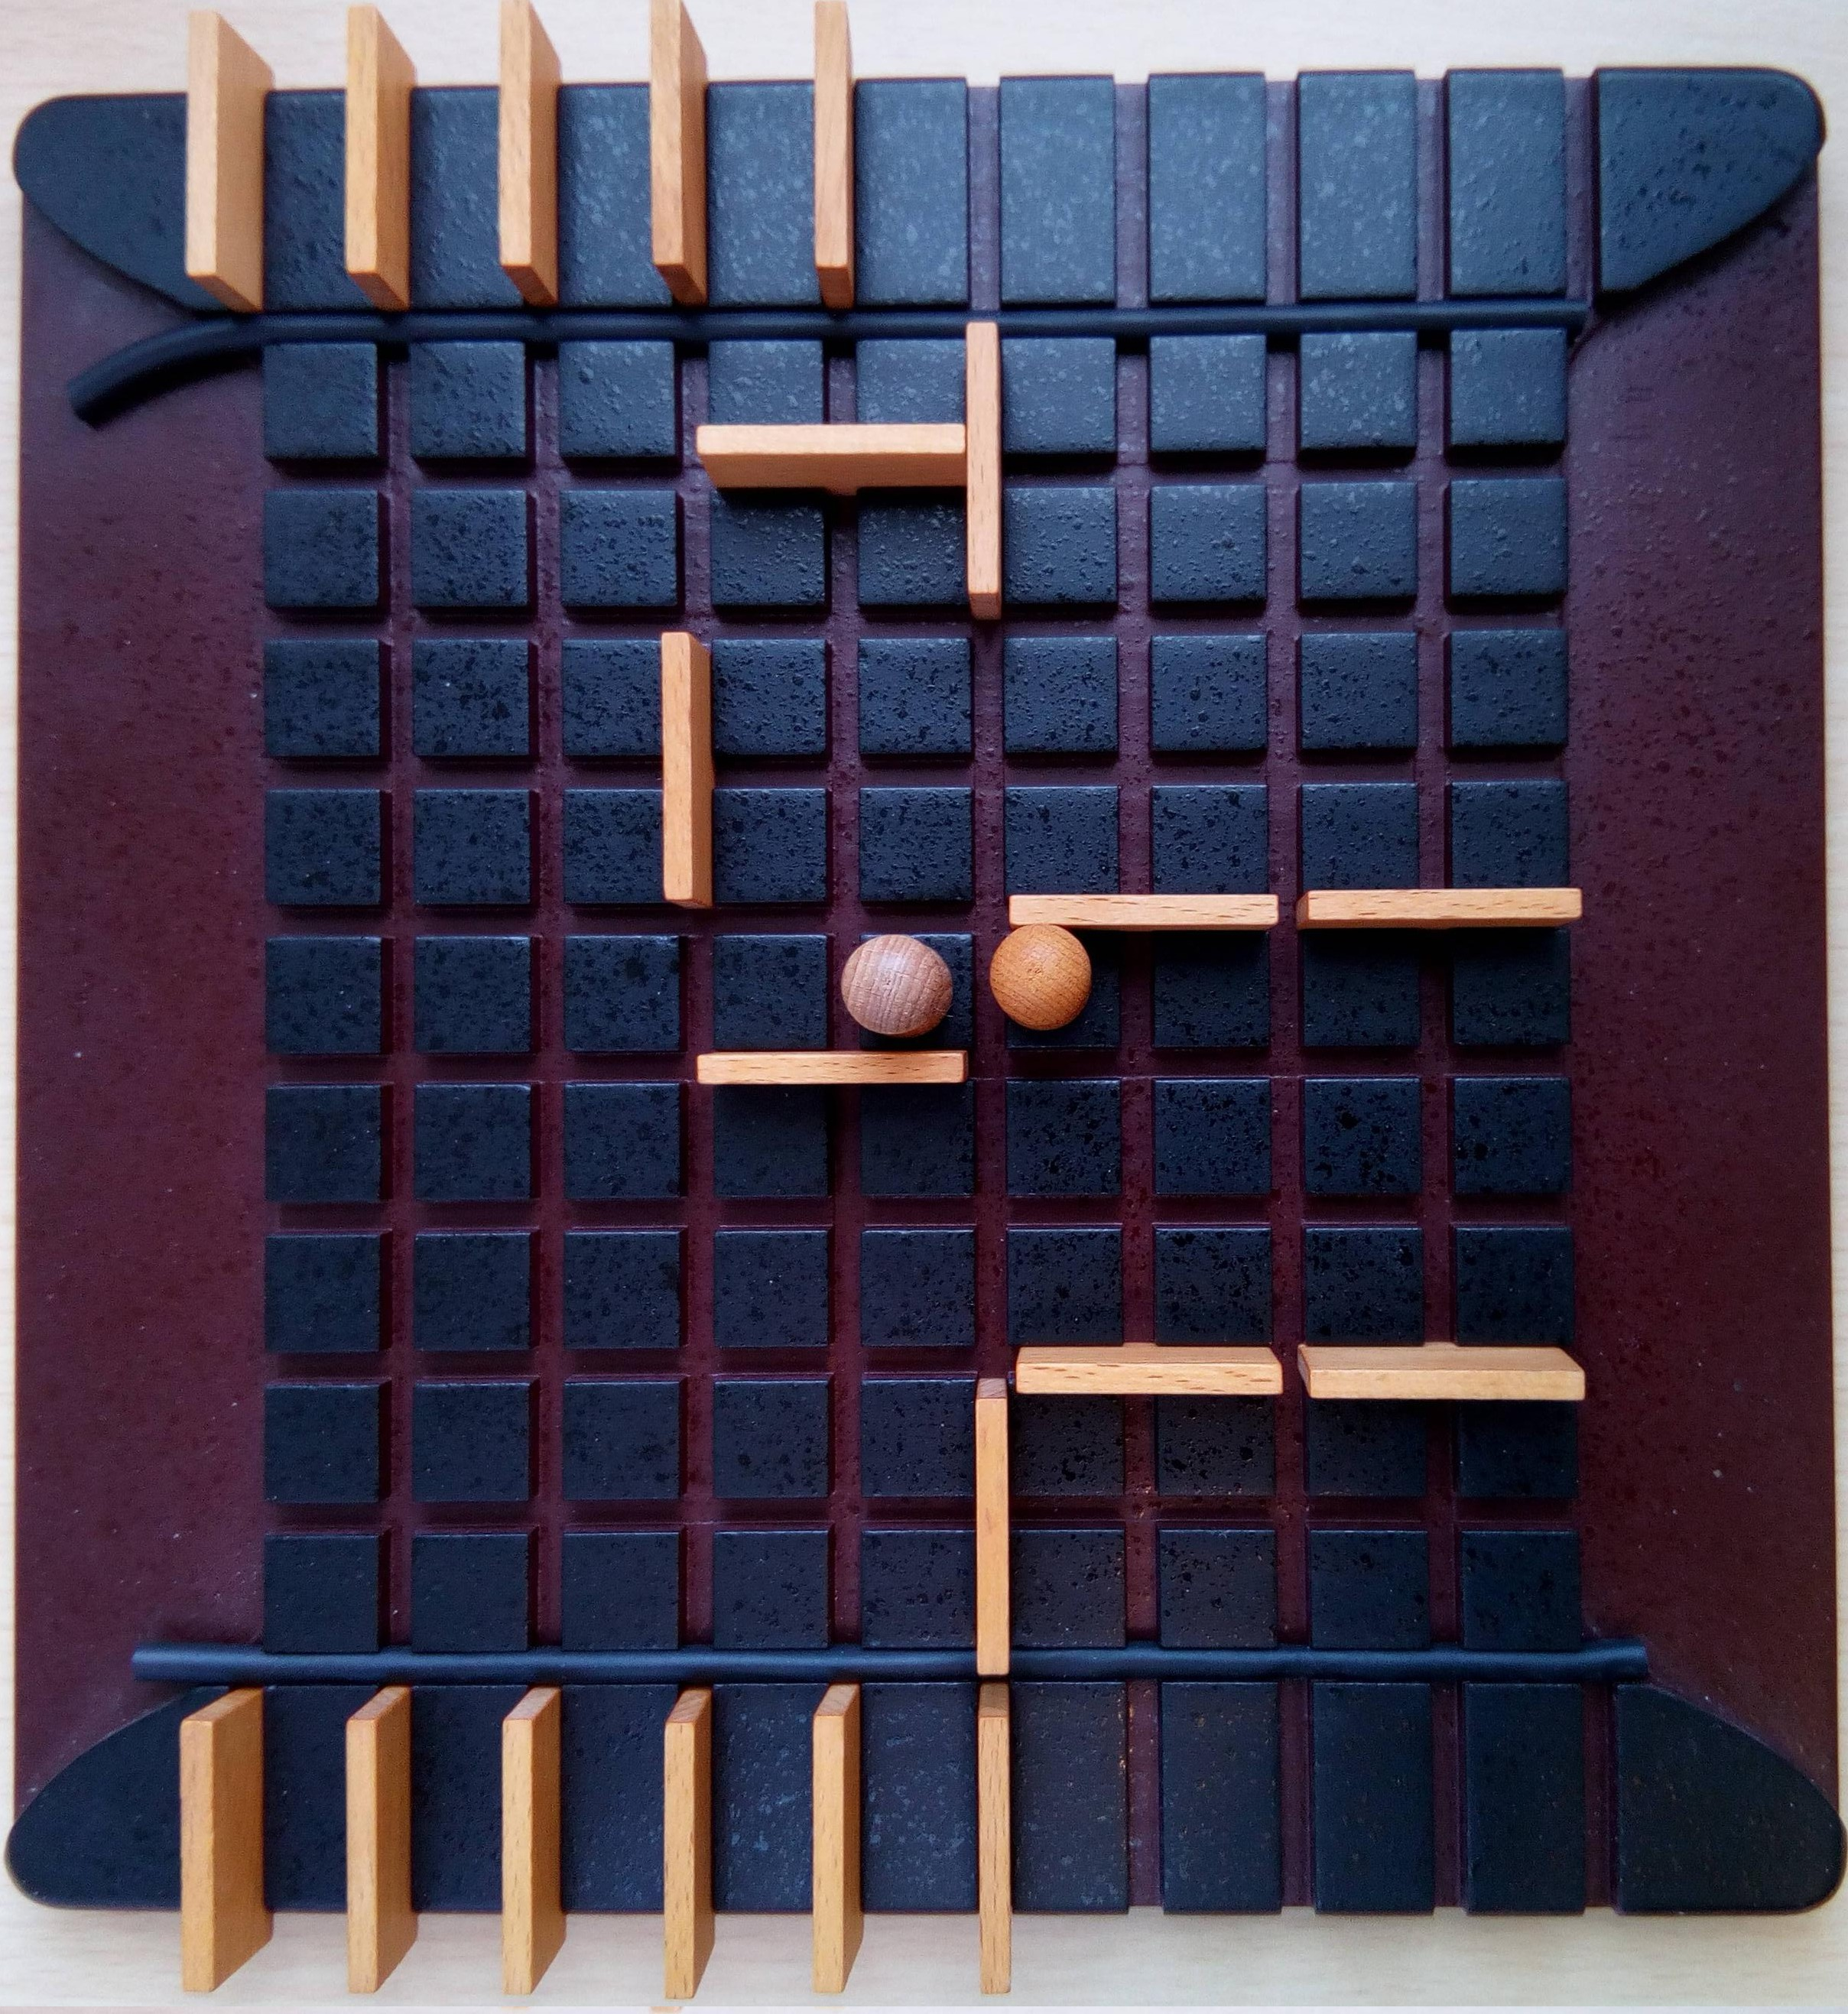
\includegraphics[width=0.35\textwidth]{real_board.jpg}
  \vspace*{-0.60cm}
  \caption{quoridor board}
  \label{fig:quoridor_board}
  \vspace*{-1.00cm}
\end{wrapfigure}

Quoridor is abstract board strategy game for 2 or 4 players with size of
9x9 (81) squares. This thesis covers 2 player version of the game.

Each player starts with a single pawn in the center of the edge on the
opposite side as the opponent.
The goal for each player is to reach the opposite edge.

\begin{wrapfigure}{L}{0.35\textwidth}
  \vspace*{-0.20cm}
  \centering
  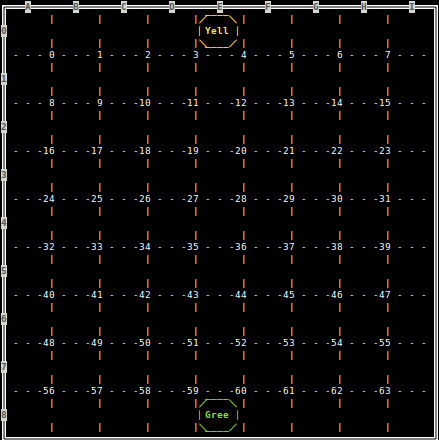
\includegraphics[width=0.35\textwidth]{start.png}
  \vspace*{-1.20cm}
  \caption{game start}
  \label{fig:game_start}
  \vspace*{-0.40cm}
\end{wrapfigure}

Player also starts with 10 walls (fences) in the stock.
Walls are two space wide and can be placed in the groove that runs between
the spaces.
Placed wall blocks pawns paths forcing them to go arount it.
Walls once placed can not be moved nor removed.
Wall can not be placed to the position already occupied or crossing by
other wall.
Also, wall can not cut off the only remaining path of any pawn to his goal.

When player is on turn, he must place wall, if he has left some, or move
his pawn to adjacent (not diagonal and unoccupied) space.
If opponent's pawn stands on an adjacent space, current player can jump
with his pawn to all the places where the opponent pawn can move.

\section{Quoridor complexity}
\begin{wrapfigure}{r}{0.52\textwidth}
  \vspace*{-2.35cm}
  \begin{equation}
    \label{eqn:mertensestimate}
    \begin{aligned}
      S_p\!&=\!81 \cdot 80 = 6480 \\
      S_f\!&=\!\sum_{i=0}^{20}\prod_{j=0}^{i}(128 - 4i)\!=\!6.1582{\cdot}10^{38} \\
      S\!&=\!S_p \cdot S_f = \mathbf{3.9905 \cdot 10 ^{42}}
    \end{aligned}
  \end{equation}
  \vspace*{-1.25cm}
\end{wrapfigure}

Estimated game state complexity was $3.9905\cdot10^{42}$
[\cite{mertens}] (equation \ref{eqn:mertensestimate}), however, this is very rough estimate, since
it includes many states multiple times where it counts with permutations
instead of combinations of walls.

Average branging factor of the game has been calculated to be $60.4$ and
average game length to be $91.1$ [\cite{glendenning}]. This Mertens used to
compute game-tree size $G = 60.4^{91.1} = 1.7884{\cdot}10^{162}$.

My approach (equation \ref{eqn:myestimate}) with estimating state complexity
will be similar. I will estimate maximum states of this game, which will
include impossible states such as:
\begin{itemize}
  \vspace*{-0.25cm}
  \setlength\itemsep{0cm}
  \item walls crossing each other
  \item pawns in the winning position and on turn
  \item pawns not having the path to the winning position
  \item pawn in the winning position where it could not end due to walls
  \vspace*{-0.15cm}
\end{itemize}
\begin{wrapfigure}{r}{0.50\textwidth}
  \vspace*{-1.90cm}
  \begin{equation}
    \label{eqn:myestimate}
    \begin{aligned}
      S_p &= 81 {\cdot} 80 - 9 {\cdot} 9 = 6399\\[-0.20cm]
      f(i)\!&=\! \begin{cases}
        i + 1  & \quad \text{if } i <= 10 \\[-0.30cm]
        21 - i & \quad \text{if } i > 10
      \end{cases}\\
      S_f\! &=\! \sum_{i=0}^{20} f(i){128 \choose i} = 1.7796 {\cdot} 10^{23}
      \\
      S &= 2 {\cdot} S_p {\cdot} S_f = \mathbf{2.2775 {\cdot} 10^{27}}
    \end{aligned}
  \end{equation}
  \vspace*{-1.15cm}
\end{wrapfigure}
Moreover, this estimate will count as a different state when different
player is on the move, and also, different number of walls in players
stocks. Both of these could make the game very different in the outcome.

$S_p$ was corrected to not include both pawns in the winning positions.
$f(i)$ % is from sequence $\{1, 2, ..., 9, 10, 11, 10, 9, ..., 2, 1\}$ and
stands for different wall counts in the stocks.
$2$ in $2{\cdot} S_p {\cdot} S_f$ counts different players on turn.

The result is maximum number of possible states, which is significantly
less then former estimate. However, even if I could evaluate $10^{6}$
states in one second, it would take around $7.2172{\cdot}10^{13}$ years to
evaluate this many states. Also, lets assume it takes on average 50B
of memory per state. Then I would need approximately
$1.1387{\cdot}10^{29}$ bytes of memory to store all states in the
computer. This is why simple Q-learning is not feasible.

